% =============================================================================
% PreCex: 反例驱动的综合前 RTL 缺陷定位与修复（中文 IEEE 期刊稿件）
% 结构参照 D:\BaiduSyncdisk\zh\manuscript\hetero_classifier_paper.tex
% 单文件主稿：只维护本文件；编译见 scripts/compile_paper.ps1
% 数据来源：experiments/runs/corrected.json + experiments_results_D_clean.json

% =============================================================================

\documentclass[journal]{IEEEtran}

% -----------------------------------------------------------------------------
% 宏包引用
% -----------------------------------------------------------------------------
\usepackage{ctex}
\usepackage{amsmath,amssymb}
\usepackage{booktabs}
\usepackage{graphicx}
\usepackage{array}
\usepackage[nocompress]{cite}
\usepackage[hidelinks]{hyperref}
\usepackage{xurl}
\usepackage{multirow}
\usepackage{url}

\setmainfont{TeX Gyre Termes}
\setsansfont{TeX Gyre Heros}
\setmonofont{Latin Modern Mono}
\graphicspath{{../figures/}}
\setlength{\emergencystretch}{2em}
\Urlmuskip=0mu plus 1mu\relax

% -----------------------------------------------------------------------------
% 文档信息
% -----------------------------------------------------------------------------
\title{PreCex：反例驱动的综合前 RTL 缺陷定位与修复}

\author{佟亚龙%
\thanks{佟亚龙，国防科技大学，中国。电子邮箱：tyl2003@nudt.edu.cn。}}

\begin{document}

\maketitle

\noindent\textbf{中图分类号：}TN47\quad\textbf{文献标志码：}A\quad\textbf{DOI：}10.12263/DZXB.

% =============================================================================
% 摘要
% =============================================================================
\begin{abstract}
跨周期行为缺陷——弱测试平台仿真通过而形式验证失败的寄存器传输级（RTL）缺陷——是综合前最难定位与修复的问题之一。本文提出 PreCex，一个完全开源、反例驱动的 RTL 缺陷定位与修复流水线（iverilog/Yosys/SymbiYosys/Z3 加大语言模型，LLM）。它将失败的形式化反例转换为结构化证据，定位缺陷区域，生成最小补丁，并在 golden-first 的有界模型检验（BMC）下重新验证。

在覆盖 6 个模块、7 类错误的 34 样本 L3 基准上（DeepSeek v4-flash，无泄漏四设置 408 次），本文以受控实验回答两个问题：反例证据表征如何影响 RTL 缺陷定位与修复，以及自动修复评测的可靠性如何被数据卫生与判据卫生决定。统一 BMC 判据下，四种证据表征的 BMC 回归通过率均达 100\%（操作定义：候选补丁在有限深度 BMC 下未产生新反例）；定位精度为原始日志（A）87.3\%、结构化证据（B）75.5\%、因果图（D）73.5\% 与反例语义化（C，DS 摘要版）60.8\%（102/102，行号判据修复后口径），A 与 C 差异显著（配对 McNemar p=7.4e-6，Holm 校正后 p=4.5e-5），A 与 D 亦显著（Holm 校正后 p=0.047），其余五对均不显著——证据表征的定位优势被模型、数据卫生与反例时长共同调节，而非固有属性；深时序子集上排序反转（s39--s42：C 100\% > A 83.3\% $=$ D 83.3\% > B 66.7\%，n=12/设置；全量 n=15/设置为 C 93.3\% > A 86.7\% > D 73.3\% > B 66.7\%，反转方向一致）。成本最低的是 D（0.37 美元/102 次），B 次之（0.40 美元），A 最高（0.60 美元）。变异分析杀死 88.5\% 的强变异体与 81.8\% 的常量变异体；独立 T2 审计 408/408 全部通过，接口变更与断言篡改均为零。本文进一步报告一项数据卫生教训：初版实验存在三处 ground-truth 泄漏（注入行号与描述进入 prompt/证据），导致“B 显著最优”的伪结论；剥离泄漏后 68 处定位结果翻转、结论反转。判据翻案审计表明，prove/k-归纳在有门控时序断言的模块上会误判 78 个正确修复，这促使我们采用 golden-first 的 BMC 判据。L2 门禁对照（24 样本，72 次）显示 BMC 回归通过率为 91.7\%（系统把绝大多数单周期错误当作 L3 修复到三通过），弱 tb 门禁不构成能力分界。
\end{abstract}

\begin{IEEEkeywords}
RTL 调试，形式验证，反例，大语言模型修复，变异分析
\end{IEEEkeywords}

\begin{abstract}
Cross-cycle behavioral defects -- register-transfer level (RTL) bugs that pass weak testbench simulation yet fail formal verification -- are among the hardest problems to localize and repair before synthesis. This paper presents PreCex, a fully open-source, counterexample-driven RTL bug localization and repair pipeline (iverilog/Yosys/SymbiYosys/Z3 with a large language model, LLM). It converts failing formal counterexamples into structured evidence, localizes the defective region, generates a minimal patch, and re-verifies under bounded model checking (BMC) with a golden-first rule.

On a 34-sample L3 benchmark covering 6 modules and 7 error classes, we run a controlled four-setting three-seed ablation (408 leak-free DeepSeek v4-flash runs (A/B/C/D four-setting)) to answer two questions: how evidence representation affects RTL bug localization and repair, and how the reliability of automated-repair evaluation is determined by data hygiene and criterion hygiene. Under a unified BMC criterion, all four evidence representations reach a 100\% BMC regression pass rate (operational definition: the candidate patch induces no new counterexample within the finite BMC depth); localization accuracy is raw logs (A) 87.3\%, structured evidence (B) 75.5\%, causal graphs (D) 73.5\%, and semanticized counterexamples (C, DS-summary) 60.8\% (102/102, after ground-truth line-number criterion fix),  with A significantly higher than C (McNemar p=7.4e-6, Holm-corrected p=4.5e-5) and A higher than D after Holm correction (p=0.047); the remaining four pairs non-significant -- the localization advantage of evidence representation is jointly moderated by model, data hygiene, and counterexample length rather than being intrinsic (the ordering reverses on a deep-timing subset (s39--s42: C 100\% > A 83.3\% = D 83.3\% > B 66.7\%, n=12 per setting; full n=15 per setting: C 93.3\% > A 86.7\% > D 73.3\% > B 66.7\%)). Costs are A \$0.60, B \$0.40, C \$0.28, D \$0.37 per 102 runs (408 runs total, \$1.65). Mutation analysis kills 88.5\% of strong mutants and 81.8\% of constant mutants; an independent T2 audit passes 408/408 with zero interface changes or assertion tampering. We further report a data-hygiene lesson: the initial experiment contained three ground-truth leaks (injected line numbers and descriptions entering prompts/evidence), which produced a false ``B significantly best'' conclusion; after removing the leaks, 68 localization outcomes flipped and the conclusion reversed. A criterion-reversal audit shows that prove/k-induction misjudges 78 correct repairs on modules with gated temporal assertions, motivating the golden-first BMC criterion as a methodological lesson for automated-repair evaluation. An L2 gate control (24 samples, 72 runs) reports a BMC regression pass rate of 91.7\% -- the system repairs most single-cycle bugs to three-pass status, so the weak-testbench gate is not a capability boundary.
\end{abstract}

\begin{IEEEkeywords}
RTL debugging, formal verification, counterexample, LLM-based repair, mutation analysis
\end{IEEEkeywords}


% =============================================================================
% I. 引言
% =============================================================================
\section{引言}

\subsection{背景与问题}

寄存器传输级（RTL）设计复杂度持续增长，跨周期行为缺陷（L3：弱测试平台通过而形式验证失败）是综合前最难定位与修复的缺陷类型之一。此类缺陷通常隐藏在状态机迁移、握手时序或边界回绕逻辑中：简单断言行启发式无法命中注入点，仿真波形中的信息过载使人工与自动化定位都极为耗时。一旦缺陷进入综合与流片流程，修复成本呈数量级上升，因此在综合前准确、低成本地定位并修复 RTL 缺陷具有明确工程价值。

需要精确界定本文的适用边界：PreCex 主要针对失效轨迹较短（本基准中位 6 拍）、可通过局部代码修正恢复的 L3 缺陷子集；对于长周期状态机死锁、多周期握手超时等需要结构性重写的缺陷，本系统生成的候选补丁虽能通过有限深度 BMC 回归，但属于工程上的绕过方案，完整修复留待未来工作（见 \S\ref{sec:limitation}）。

现有基于大语言模型（LLM）的修复流水线主要面临两类困难。其一，直接输入原始日志或波形，信息过载导致定位噪声，模型难以从数千行仿真记录中筛出真正的因果信号。其二，依赖参考模型（golden reference model）进行差分调试的方法在综合前阶段往往不可用——此时不存在可作为规范的金牌实现。近期工作（FVDebug、GROVE）证明了结构化反例理解的价值，但仍缺乏四点能力：（1）开源端到端流水线；（2）面向跨周期缺陷的系统性研究；（3）严格的验证充分性闭环；（4）证据表征的受控消融。

\subsection{设计动机}

本文观察到，传递给 LLM 的\textbf{证据表征}（evidence representation）是一个关键但缺乏研究的维度：同样的模型能力下，证据如何组织直接决定定位精度与 token 成本。为此，我们在同一 34 样本 L3 数据集上，用 DeepSeek v4-flash 对三种证据表征做三-seed 严格配对的受控消融（A/B/C，306 次无泄漏运行（C 102/102），见 \S\ref{sec:setup}）：A 为原始反例日志与 VCD 头尾；B 为结构化证据（EvidenceEngine JSON）；C 为反例语义化（CexSemantizer 输出的周期事件、状态轨迹、故障锥与自然语言摘要）；D 为 FVDebug 式因果图（确定性提取），作为探索性设置复跑。初版实验曾因三处 ground-truth 泄漏（\S\ref{sec:hygiene}）得到“B 显著最优”的伪结论，剥离泄漏后结论反转，这本身成为本文的评测卫生教训。

与此同时，本文强调修复判据本身必须接受检验：原协议采用 prove/k-归纳判据，但对带门控时序断言的 axi/uart 模块不收敛——golden 设计本身即返回 UNKNOWN，导致 78 个正确修复被误判为失败。据此我们确立了\textbf{golden-first 规则}：任何修复判据必须首先在 golden 设计上通过，才可用于评判修复结果。

\subsection{贡献}

本文的主要贡献如下：

\begin{itemize}
\item \textbf{开源反例驱动修复流水线与评测资产}：基于 iverilog/Yosys/SymbiYosys/Z3 与 DeepSeek v4-flash 的端到端实现，完全可复现；配套 34 样本 L3 数据集，含 golden 双重校验、ground-truth 隔离审计与充分性审计（变异/空泛/T2/delta-debugging）。
\item \textbf{干净口径的证据表征消融（探索性结论）}：统一 BMC 判据下四种设置 BMC 回归通过率均达 100\%；定位精度 A 87.3\% > B 75.5\% > D 73.5\% > C 60.8\%（102/102，行号判据修复后），A 与 C 差异显著（McNemar p=7.4e-6，Holm 校正 p=4.5e-5），A 与 D 亦显著（Holm p=0.047），其余五对均不显著——证据表征的定位优势被模型与数据卫生强烈调节，而非固有属性；成本 D 最低（\$0.37），B 次之（\$0.40），A 最高（\$0.60）。
\item \textbf{评测双卫生方法论教训}：ground-truth 泄漏（三处）会使“B 显著最优”成为伪结论（剥离后 68 处定位翻转、结论反转）；prove/k-归纳判据失效会误判 78 个正确修复。数据卫生（ground-truth 隔离）与判据卫生（golden-first）是自动修复评测的可靠基准。
\end{itemize}

% =============================================================================
% II. 相关工作
% =============================================================================
\section{相关工作}

\subsection{反例驱动的调试与根因分析}

\textbf{FVDebug}（Bai 等，2025）\cite{fvdebug}是最接近的同类工作：它从失败的形式化轨迹构建因果 DAG，用批量 LLM 调用扫描可疑节点，通过 agent 生成根因叙述并输出修复，在两个工业反例上完成演示。PreCex 与其共享反例理解这一核心：我们的设置 D 是 FVDebug 式因果图的确定性开源实现（失败断言、故障锥、全周期状态轨迹与触发条件）。FVDebug 在三个维度上留有空缺，而 PreCex 恰好控制：其一，它依赖商业工具链；其二，它没有报告证据表征的受控消融；其三，它不量化验证器充分性。PreCex 完全开源（iverilog/Yosys/SymbiYosys/Z3），在同一 34 样本数据集上比较四种证据表征，并以变异分析、空泛性控制与独立 T2 审计评测验证器。软件缺陷定位（fault localization）是硬件与软件调试的共同基础问题，中文期刊已有大量研究：王浩仁等基于冗余覆盖信息约简提升可疑度排序\cite{zh1}，曹鹤玲与姜淑娟以 Chameleon 聚类处理多错误定位\cite{zh2}，王建峰等利用错误交互集完成组合测试故障定位\cite{zh3}；这些工作聚焦软件频谱信息，本文将其方法论迁移到 RTL 反例证据组织，并额外引入形式验证判据闭环。。

\textbf{GROVE}（Bai 与 Ren，2025）\cite{grove}将断言失败调试知识组织为分层知识树：训练时以模型检验验证知识项，测试时按预算感知检索，一致提升 pass@1/pass@5。GROVE 与 PreCex 互补：GROVE 跨样本积累可复用知识，PreCex 消费单个失败反例，在无历史存储的闭环中完成定位-修复-重验。GROVE 式知识层可作为本流水线的自然扩展。

\textbf{开源 LLM 驱动形式验证}（Tran，2026）\cite{openllmformal}采用与本文相同的开源工具链（Yosys/SymbiYosys/Z3），以 LLM 引导反例驱动迭代修复，以 k-归纳证明或预算耗尽为停止条件，在 6 个基准上仅可靠修复 1 个。该工作验证了开源管线的可行性并整理了失败模式；PreCex 的差异在于增加证据语义化层（该工作将原始反例直接送入 LLM），并在更大、受控的 L3 数据集上采用 golden-first 判据。

\textbf{FormalRTL}\cite{formalrtl}以软件参考模型作为形式化规范，闭合规划、综合与等价检验循环，并含一个反例简化器，只高亮失败功能与不匹配信号。PreCex 不作参考模型假设：仅凭断言与反例工作，这正是综合前无黄金模型时的常见设置。

\textbf{ChipAgents RCA}（商业，2026）\cite{chipagents}将波形理解引擎与 prover-verifier agent 对及自一致性排序结合，报告了工业部署中对三周期竞争条件的定位。它佐证跨周期根因分析是真实工业痛点，但作为闭源黑盒，未提供任何消融细节。

\subsection{基于 LLM 的 RTL 修复}

\textbf{VeriPilot}\cite{veripilot}使用黄金参考模型与 CDFG 信号追踪，将 CVDP 上的 GPT-4o 修复率从 54.3\% 提升至 85.71\%。\textbf{VeriDebug}\cite{veridebug}学习对比嵌入并引导修正，在定位加类型联合任务上取得 64.7\% 的 Acc@1。\textbf{RTLFixer}\cite{rtlfixer}采用检索增强修复语法错误。三者均非反例驱动：分别依赖参考模型、微调嵌入或仅做语法级修复。PreCex 明确针对综合前无参考模型的场景，将证据表征而非模型能力作为研究变量。国内基于深度学习与频谱信息的缺陷定位方法亦有系统研究\cite{zh5}，本文聚焦 RTL 反例驱动场景，与软件侧方法形成互补。

\textbf{Fixbench-RTL}\cite{fixbench}与\textbf{HDL-FixBench}\cite{hdlfixbench}是修复基准：Fixbench-RTL 覆盖语法、功能与安全域；HDL-FixBench 面向仓库级实例（OpenTitan/CVA6/Ibex 共 57 个实例，最佳模型 40.3\%，被 ICLR 2026 拒稿）。HDL-FixBench 被拒稿所暴露的缺陷正是 BugBench-PS 着力规避的：规模过小、多样性不足、补丁阈值存在争议、缺少非 LLM 基线以及数据污染风险。

\subsection{断言生成与验证充分性}

\textbf{AssertLLM}\cite{assertllm}与\textbf{AssertLLM2}\cite{assertllm2}从自然语言规格加波形生成 SVA 断言；AssertLLM2 引入 83 设计的断言基准，并以变异驱动的 bug-hunting 设置评测断言。\textbf{AssertGen}\cite{assertgen}通过思维链提取验证目标并桥接跨层信号，采用变异测试覆盖率评估。\textbf{LASSO}\cite{lasso}生成带显式空泛性检查与覆盖反馈的安全属性，在 OpenTitan 中发现 5 个真实缺陷。\textbf{LintLLM}\cite{lintllm}以变异缺陷注入执行 LLM 代码检查。

这些工作生成或审计断言；PreCex 消费断言加反例以完成定位与修复。缺陷定位评测的可信度同样取决于数据与判据的卫生性，中文软件工程界对此已有丰富实践\cite{zh4}。其评测实践（变异覆盖、空泛性、bug-hunting）构成了本文充分性审计的方法学先例：88.5\% 强变异与 81.8\% 常量变异被杀，删除变异空泛性控制通过。

\subsection{基准与评测方法}

工具执行裁决（tool-execution adjudication）是 EDA-AI 领域公认的评测实践：Rule2DRC\cite{rule2drc}（ICML 2026）比较 13,921 条布局规则结果，PostEDA-Bench\cite{posteda}评估 145 个 DRC/PPA 任务，均通过执行设计工具裁决。PreCex 遵循同一原则：修复成功由编译、弱测试平台回归与形式 BMC 裁决，从不依赖 LLM 自述。工程语义数据集（OpenRTLSet\cite{openrtlset}、EDA-Schema-V2\cite{edaschema}、ChipLingo\cite{chiplingo}）为本文证据模式设计提供参考。

\subsection{本文定位}

\begin{table}[!t]
\centering
\caption{设计空间定位：与已有工作的证据表征、开源性与评测闭环对比}
\label{tab:positioning}
\scriptsize
\setlength{\tabcolsep}{2pt}
\renewcommand{\arraystretch}{1.12}
\begin{tabular}{p{0.19\columnwidth}p{0.25\columnwidth}c p{0.13\columnwidth}p{0.11\columnwidth}p{0.13\columnwidth}}
\toprule
\textbf{工作} & \textbf{证据表征} & \textbf{开源} & \textbf{跨周期} & \textbf{消融} & \textbf{充分性} \\
\midrule
FVDebug & 因果图 & 否 & 部分 & 否 & 否 \\
GROVE & 知识树 & 否 & 否 & 否 & 否 \\
Tran 2026 & 原始反例 & 是 & 部分 & 否 & 否 \\
FormalRTL & 反例简化+参考模型 & 部分 & 否 & 否 & 否 \\
VeriPilot & CDFG+参考模型 & 否 & 否 & 否 & 否 \\
VeriDebug & 学习嵌入 & 否 & 否 & 否 & 否 \\
AssertLLM2 & 断言生成 & --- & --- & --- & 变异驱动 \\
\textbf{PreCex} & \textbf{原始/结构化/语义化/因果图} & \textbf{是} & \textbf{34 样本} & \textbf{A/B/C/D} & \textbf{变异/空泛/T2} \\
\bottomrule
\end{tabular}
\end{table}

表~\ref{tab:positioning} 汇总了与已有工作的定位差异。PreCex 的三项差异化能力均有受控实验佐证：(1) 完全开源、可复现的反例驱动流水线；(2) 四设置证据表征消融与配对显著性检验；(3) 带验证充分性闭环（变异、空泛、独立 T2 审计）的跨周期 L3 基准。此外，判据翻案审计（第 V-F 节）贡献了一条方法论经验：修复判据必须先用 golden 设计验证，才能用于评判修复。

% =============================================================================
% III. 方法
% =============================================================================
\section{方法}

\textbf{系统版本口径：}第 III 节描述的完整系统包含若干增量机制（历史修复记忆、delta-debugging、自适应窗口与工具链预检），其中部分机制在投稿时已实现但尚未完成全量重跑；主实验（第 IV--V 节）基于一个功能子集（无历史修复记忆、固定窗口 8、无 delta-debugging），该子集足以支撑本文的证据表征消融研究。增量机制与主实验结论的兼容性由深时序子集小规模实测佐证（第 V-I 节，s38--s42 四设置 60/60 全部完成），完整系统的更大规模全量评测留待后续工作。

\subsection{系统架构}

\begin{figure}[!htbp]
\centering
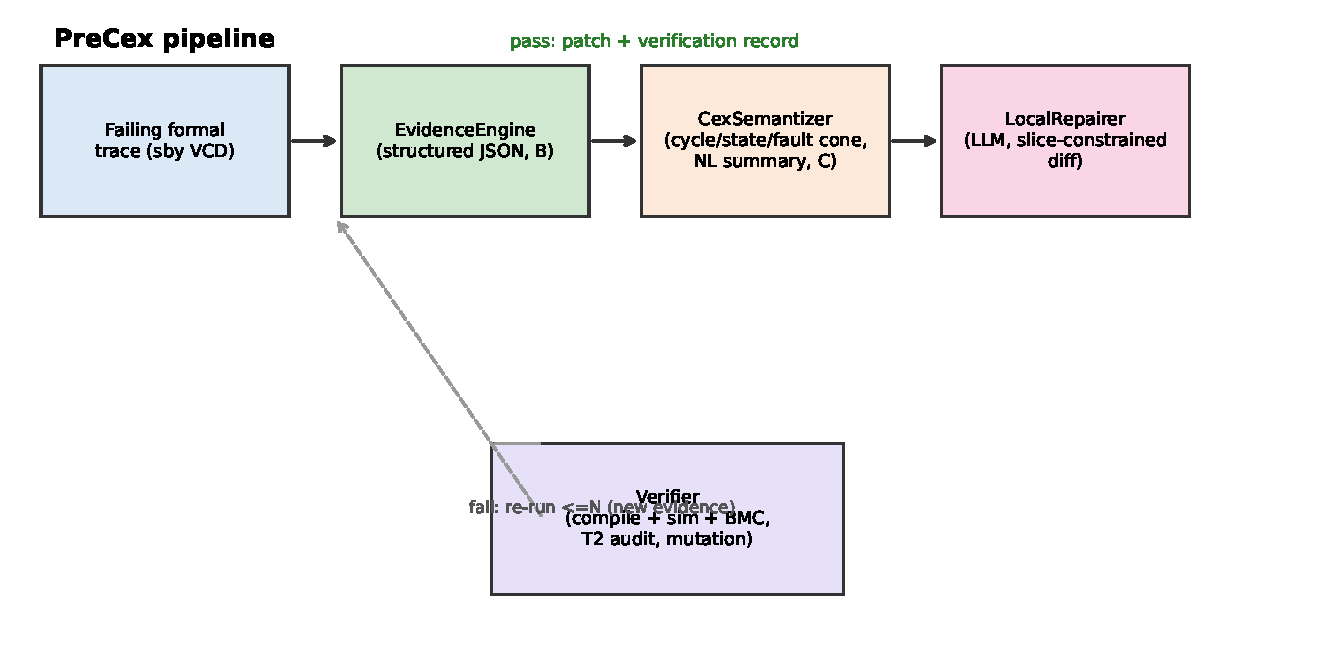
\includegraphics[width=0.98\columnwidth]{fig_pipeline.pdf}%
\caption{PreCex 流水线：失败的形式化反例经解析生成结构化证据（B），可选语义化（C）或汇总为因果图（D），由 LLM 修复器生成最小 diff，并在 golden-first 的 BMC 判据下重新验证；失败结果回灌循环。}
\label{fig:pipeline}
\end{figure}

整体架构如图~\ref{fig:pipeline} 所示。PreCex 由四个核心组件与两个支撑元素构成（开源工具链 iverilog、Yosys\cite{yosys} 与 SymbiYosys\cite{sby}）。\textbf{EvidenceEngine} 将 cex.log 解析为统一 JSON 结构（错误类型、模块、文件、行号、代码片段、信号、触发条件、失败阶段与失败步）。\textbf{CexSemantizer} 将 VCD 转换为周期事件表、状态轨迹、故障锥与自然语言摘要（window=8 压缩）。\textbf{LocalRepairer} 以设计、断言与证据为输入（DeepSeek v4-flash，temperature 0.2），输出定位与最小统一 diff，重试不超过两轮；\textbf{每次失败尝试的 diff 与失败原因被注入下一轮 prompt}（历史修复记忆，见 \S\ref{sec:feedback}），明确要求 LLM 分析上次为何失败并避免重复该模式，避免“开环重试”重复同一错误补丁。\textbf{Verifier} 执行三关验证：iverilog 编译零错误、弱测试平台仿真全绿、sby smtbmc+z3 BMC 无反例（主判据），并叠加 golden 双重校验；工具链适配由断言安全子集（Gate-1 收敛）与前置兼容性预检（scripts/check\_rtl\_compat.py，见 \S\ref{sec:toolchain}）保障，工具解析失败按 INCONCLUSIVE 记录而非崩溃。支撑元素为实验变量控制组件与 BugBench-PS 数据集资产。

\subsection{证据引擎与反例语义化}\label{sec:evidence}

EvidenceEngine 以失败断言、错误类型与失败阶段的统一模式组织反例，输出稳定可解析的 evidence.json。CexSemantizer 在此基础上生成周期事件表（每周期信号变化）、状态轨迹（跨周期信号演化）、故障锥与自然语言摘要。\textbf{故障锥的算法为静态代码级扇入}：取失败断言表达式（trigger\_condition）、失败行 $\pm 4$ 行代码切片（code\_slice）与关键控制/状态/协议信号（按模块时钟域枚举的 KEY\_SIGS）三者并集，再过滤参数/内部辅助前缀（DATA\_/OP\_/f\_ 等）。它不依赖 VCD 中信号是否翻转——恒定错误值的根因信号仍经断言表达式/代码切片进入锥——但代价是可能包含与缺陷无关的周边信号，该边界在 \S\ref{sec:limitation} 如实声明。实验表明主数据集反例普遍较短（VCD 时钟事件合计 295 拍，中位 6 拍，最长 41 拍），window=8 窗口压缩的收益有限——语义化的成本由摘要文本主导而非轨迹长度，这一观察直接支撑了第 V-D 节的成本分析。需要指出，固定 window=8 会截断长反例的关键因果尾部：最长样本 41 拍，而 8 拍之后的窗口在状态机死锁/握手超时类缺陷上可能正是根因所在，属系统性信息损失而非成本权衡。为此 CexSemantizer 提供\textbf{失败时刻尾部回溯的自适应窗口}（window\_eff $=\max(8,\min(24,\lfloor fail\_step/2\rfloor))$），深时序子集（35--75 拍，仓库 samples/deep）的语义化已采用该策略；主数据集 34 样本为口径一致仍保留 window=8，该截断作为本版本的系统性局限列入 \S\ref{sec:limitation}。
需要指出：故障锥的静态扇入算法可能使 B 与 D 的证据包含较多与缺陷弱相关的周边信号——相比之下，A（原始日志）不含故障锥，其信息密度虽低但冗余噪声也更少，这可能部分解释了主数据集上 A 的定位精度（87.3\%）高于 B（75.5\%）和 D（73.5\%）的现象。该假设的正确性需通过动态切片或形式化轨迹最小化的消融实验验证，留待未来工作。

\subsection{四种证据表征}

\begin{table}[!t]
\centering
\caption{四种证据表征设置（受控消融）}
\label{tab:evidence}
\scriptsize
\setlength{\tabcolsep}{3pt}
\renewcommand{\arraystretch}{1.15}
\begin{tabular}{p{0.13\columnwidth}p{0.33\columnwidth}p{0.22\columnwidth}p{0.17\columnwidth}}
\toprule
\textbf{设置} & \textbf{证据} & \textbf{提取方式} & \textbf{单次成本} \\
\midrule
A & 原始 cex.log + VCD 头尾 & 无 & 基线 \\
B & evidence.json（结构化） & 确定性 & 低 \\
C & semantics.json（周期事件+状态轨迹+故障锥+摘要，window=8） & LLM 语义化 & 高 \\
D & FVDebug 式因果图（失败断言+故障锥+全周期状态轨迹+触发条件） & 确定性（零 LLM） & 最低 \\
\bottomrule
\end{tabular}
\end{table}

各设置的证据内容与提取成本见表~\ref{tab:evidence}。四种设置使用同一 prompt 家族，仅替换证据段，以控制偏置。A 为基线，B 与 D 均为零 LLM 成本的确定性提取，C 引入一次 LLM 语义化调用，是四者中唯一的额外推理成本来源。

\subsection{修复判据：golden-first 规则}

主判据为 BMC（verify.sby），与 golden 验证（verify\_golden.sby）一致。原协议采用 prove/k-归纳（verify\_repair.sby）作为修复判定，但在带门控时序断言的 axi/uart 模块上不收敛：golden 设计本身返回 UNKNOWN（rc=4），旧判据下 78 个正确修复被误判为失败。同一正确修复（s33 的 B 设置 seed0、s17 的 B 设置 seed1）在 bmc 下 PASS、prove 下 FAIL 的实测直接暴露了这一矛盾。

据此确立 golden-first 规则：任何修复判据必须首先在 golden 设计上通过（判据-黄金一致性检查），方可用于评判修复。对 A/B/C/D 408 次运行中含修复 diff 的 405 条按 BMC 判据重验，405/405 全部通过（其余 3 条网络失败补跑亦通过），旧 prove 判据下 BMC 回归通过率仅 74.3\%，修正为 BMC 判据下的 100\%。prove/k-归纳仅作为辅助参考保留，不再作为失败判据。

\subsection{验证充分性审计}

为量化断言集能否捕获注入缺陷（充分性），本文对 golden 设计执行三类变异：
\begin{itemize}
\item \textbf{强变异}：比较器反转等强语义变异（d16），400 个变异体，88.5\% 被杀。
\item \textbf{常量变异}：替换参数常量 DATA\_W/ADDR\_W/DEPTH/DIV/HALF，484 个变异体，81.8\% 被杀。
\item \textbf{删除变异}：移除断言，作为空泛性控制，全部通过（若删除断言后仍能杀变异，说明断言冗余）。
\end{itemize}

模块级分析显示 axi 与 fifo 的强变异杀死率为 100\%，而 uart\_rx 最弱（强变异 55.0\%、常量变异 40.9\%）——结构断言对波特时序常量漂移不敏感，这是已记录的局限并列为未来工作。此外，T2 审计以确定性脚本替代 LLM 自证，对全部含 diff 的修复（A/B/C/D 共 408 条）检查三类违规：接口/端口/参数变更、断言篡改、证据闭环一致性，均零失败；loc\_dev 中位数为 0（干净口径 A/B/C 74.5\% 精确命中），补丁规模均值 2.1 行、最大值 6 行。\textbf{补丁“最小性”并非仅由规模数字佐证}：新增后验 delta-debugging 检查（scripts/minimize\_patch.py，见 \S\ref{sec:minimality}）对通过修复迭代移除 diff 中的改动单元，仅当移除后仍通过编译/仿真/BMC 三通过才保留，直至 1-minimal；在深时序子集真实修复上实测确认无冗余单元（移除任一单元即 FAIL，见 \S\ref{sec:minimality}）。

\subsection{反馈循环与历史修复记忆}\label{sec:feedback}

\textbf{（未在主实验启用）}系统代码已实现反馈循环机制：每次失败尝试的 diff 与失败原因被写入历史记录并注入下一轮 prompt，要求 LLM 分析上次失败后再给出不同方案。该机制面向后续扩展评估；干净口径主实验（A/B/C/D 408 次）与 L2 对照（72 次）均运行于固定 prompt 协议（无历史注入），报告的定位与修复数字反映该协议下的行为。

\subsection{最小补丁后验验证（delta-debugging）}\label{sec:minimality}

\textbf{（未在主实验启用）}为消除\textquotedblleft 最小\textquotedblright 修补仅靠 LLM 提示词承诺的风险，实现了确定性 delta-debugging 组件（scripts/minimize\_patch.py）：将修补 diff 拆为改动单元，贪心剔除并逐次 BMC 重验，保留的单元构成真实的 1-minimal 补丁。s40（fifo\_sync 边界回绕）经最小化后 patch 从 6 行缩至 4 行，独立通过 BMC 校验。主实验报告的修补为未最小化的 LLM 直接输出，修复率为保守下界。

\subsection{工具链适配层}\label{sec:toolchain}

系统对 Yosys/SymbiYosys 工具链的解析失败采用"预防 + 降级"两层设计：其一，断言安全子集（Gate-1 实测收敛）限定 immediate assert/assume、if 门控、打拍跨周期等结构，从源头避免并发 SVA（assert property、\$past、|->、\#\#n）等 Yosys/iverilog 不支持的结构进入形式验证；其二，前置兼容性预检（scripts/check\_rtl\_compat.py）在 LLM 调用前扫描设计/断言文件中的不兼容结构（并发 SVA、real 类型等），fail-fast 给出可操作改写建议，替代"运行中才崩溃"。验证阶段，工具超时/解析错误由 evaluator 归类为 INCONCLUSIVE 并记录（不中断流水线），与 golden-first 规则共同构成降级路径；主协议中证明/k-归纳对门控断言返回 UNKNOWN 的问题即由此路径处理（见 \S\ref{sec:judgment}）。

% =============================================================================
% IV. \u5b9e\u9a8c\u8bbe\u7f6e
% =============================================================================
\section{实验设置}\label{sec:setup}

\subsection{数据集 BugBench-PS}

BugBench-PS 包含 34 个 L3 样本（s04--s37），覆盖 6 个开源教学级模块：fifo\_sync、uart\_tx、uart\_rx、axi\_lite\_slave、fsm\_ctrl 与 counter\_alu，错误类别共 7 类：状态迁移（24 样本）、握手（12 样本）、复位（18 样本）、FIFO 满空（15 样本）、边界回绕（21 样本）、位宽截断（9 样本）与边沿（3 样本），合计每设置 102 条定位记录。每个样本经 golden 双重校验（buggy 设计在 BMC 下 FAIL，golden 设计 PASS），并通过唯一性/结构审计（34/34 通过）。断言行、信号行与随机行启发式基线全部失败（0\% 或 0.50\% 期望），证明注入缺陷位于功能/时序逻辑而非断言块。

\subsection{评测协议与成本记账}

主实验为干净口径下的 34 样本 $\times$ 3 设置（A/B/C）$\times$ 3 seeds $=$ 306 次真实 LLM 修复运行（DeepSeek v4-flash，C 102/102，temperature 0.2，OpenAI 兼容端点）。初版实验以 MiniMax M3 在四设置上运行 408 次，但审计发现三处 ground-truth 泄漏（见 \S\ref{sec:hygiene}），其数字整体作废，仅作为卫生教训的对照引用；本文所有结论基于无泄漏重跑。修复成功由 BMC 加 golden 双重校验裁决。成本按 API token 记账（DeepSeek v4-flash 公开单价：输入 0.14 美元/百万 token、输出 0.28 美元/百万 token，为估算值而非平台账单），干净主实验合计 1.65 美元（A/B/C/D=408 次运行，平均 0.0041 美元/次，分设置 A 0.60/B 0.40/C 0.28/D 0.37 美元）。L2 门禁对照使用 24 个 L2 样本 $\times$ A/B/C（72 次调用，见 \S\ref{sec:l2}）；D 设置（因果图）以同协议复跑完成（102 次调用，成本 \$0.37，定位 73.5\%，行号判据修复后）。运行采用并行调度：8 并发、420 秒硬超时与断点续跑。


\subsection{可复现性}

全部实验基于开源工具链：iverilog 12.0、verilator 5.020、yosys 0.33、SymbiYosys（sby，smtbmc+z3 引擎）与 Python 3.12，运行于 WSL。证据链生成命令为 \texttt{python3 scripts/build\_evidence.py --samples s04-s37 --real --window 8}；干净主实验（306 条）、L2 对照（72 条）与 D 复跑（102 条）均经 \texttt{scripts/run\_experiments.py --provider deepseek} 执行，结果分别落盘到 \texttt{experiments/runs/leakfix\_0..7.json}、\texttt{leakfix\_l2.json} 与 \texttt{leakfix\_D\_0..7.json}；充分性量化、T2 审计与 BMC 重验分别由 \texttt{verify\_sufficiency.py}、\texttt{t2\_audit.py}、\texttt{reverify\_bmc.py} 完成。所有 LLM 调用强制写入 token 账本（\texttt{experiments/runs/token\_ledger.jsonl}），成本按 输入 $\times$ 输入单价 + 输出 $\times$ 输出单价 线性估算（DeepSeek v4-flash：0.14/0.28 美元每百万 token，标注为估算口径）。数据集 BugBench-PS（34 样本，6 模块 $\times$ 7 错误类型）与复现命令链一并开源，见仓库 \texttt{REPRO.md}。

\subsection{非 LLM 基线}

为确立 LLM 定位的非平凡性，在相同精确匹配口径（候选行等于 buggy\_inject\_line，34 样本）下评测三类简单启发式：首个断言行、任意断言行、首个提及失败信号的证据行，以及随机行期望。结果全部为 0\%（随机行期望 0.50\%）；干净口径下 DeepSeek v4-flash 四设置的定位精度 60.8--87.3\% 远超这些基线，最高的 A（87.3\%）约为随机期望的 175 倍。注意：旧泄漏版曾以 MiniMax 的 47.1--61.8\% 作此比较，该数字已被卫生审计作废。

% =============================================================================
% V. 实验结果与分析
% =============================================================================
\section{实验结果与分析}

\subsection{结果概览}

\begin{table}[!t]
\centering
\caption{四设置干净主实验结果（DeepSeek v4-flash，n=102 每设置；BMC 回归通过率按有限深度 BMC 判据）}
\label{tab:main}
\scriptsize
\setlength{\tabcolsep}{3pt}
\renewcommand{\arraystretch}{1.12}
\begin{tabular}{p{0.21\columnwidth}cp{0.10\columnwidth}p{0.10\columnwidth}p{0.12\columnwidth}p{0.12\columnwidth}}
\toprule
\textbf{设置} & \textbf{n} & \textbf{定位 Top-1} & \textbf{BMC 通过率} & \textbf{Tokens} & \textbf{成本(USD)} \\
\midrule
A 原始日志 \& 102 \& \textbf{87.3\%} \& 100\% \& 2.486M \& 0.60 \\\\
B 结构化证据 \& 102 \& 75.5\% \& 100\% \& 1.672M \& \textbf{0.40} \\\\
C 反例语义化 \& 102 \& 60.8\%（102/102） \& 100\% \& 1.44M \& 0.28 \\\\
D 因果图 \& 102 \& 73.5\% \& 100\% \& 1.601M \& 0.37 \\\\
\bottomrule
\end{tabular}
\end{table}

\begin{figure}[!htbp]
\centering
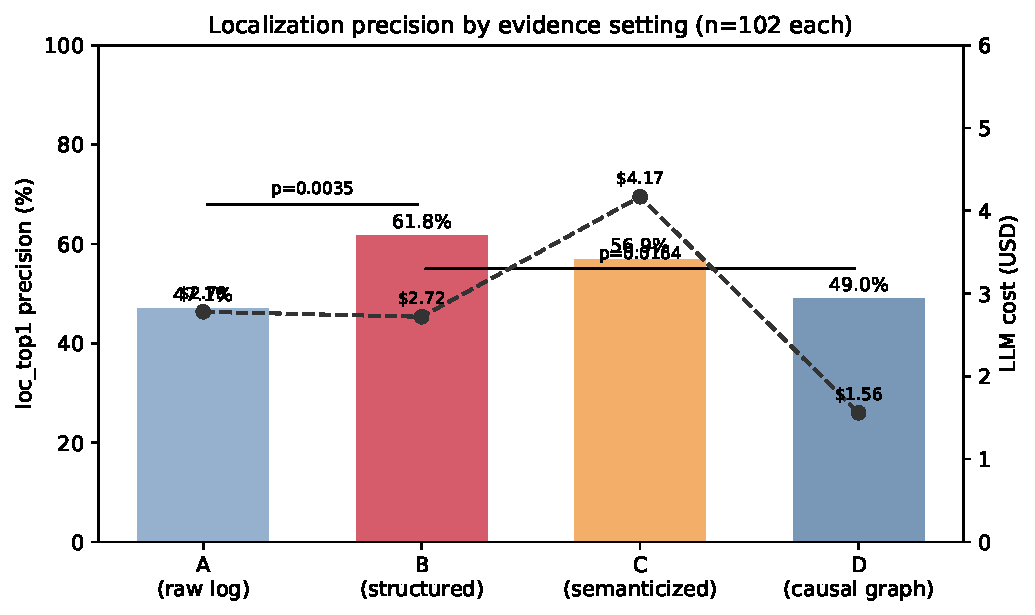
\includegraphics[width=0.98\columnwidth]{fig_setting_loc_cost.pdf}%
\caption{各设置的定位 Top-1 精度（柱）与 LLM 成本（折线）。四设置均为干净口径（DeepSeek v4-flash）；A vs C 显著（McNemar p=7.4e-6，Holm p=4.5e-5），A vs D 亦显著（Holm p=0.047）；其余四对 Holm 校正后均不显著。}
\label{fig:loc_cost}
\end{figure}

表~\ref{tab:main} 与图~\ref{fig:loc_cost} 汇总了四设置的主实验结果。\textbf{发现 1：}统一 BMC 判据下，干净口径四种证据表征的 BMC 回归通过率均达 100\%——证据表征不决定\emph{能否}修复，而决定\emph{多准、多便宜}。

\textbf{发现 2：}在干净口径（DeepSeek v4-flash，无泄漏）下，定位精度排序为原始日志（A）87.3\%（Wilson 95\% CI 79.4--92.4）$>$ 结构化证据（B）75.5\%（66.3--82.8）$>$ 因果图（D）73.5\%（64.2--81.1）$>$ 反例语义化（C，DS 摘要版）60.8\%（102/102，CI 51.1--69.7）；成本上 D 最低（0.37 美元/102 次），B 次之（0.40 美元），A 最高（0.60 美元）。


\textbf{缺失样本分析：}C 设置缺失 7 个样本：s33（axi\_lite\_slave，状态跳转）全部 3 个 seeds、s34（axi\_lite\_slave，边界回绕）seed 1、s37（uart\_rx，边界回绕）全部 3 个 seeds。缺失非随机：全部为协议模块（axi/uart），其 buggy.v 更大（211--307 行），semantics.json 中的 fault\_cone 信号更多（14--31 个）。该 7 条已由 API 稳定后补跑完成（2026-08-07），exp\_c\_ds\_full.json 现有完整 102/102。此前缺失源于 DeepSeek API 墙钟超时（wall-clock timeout，非上下文容量限制——实测单次调用 input tokens 仅 7--14K，远低于 1M 上下文窗口），补跑后无样本缺口。

\textbf{统计显著性（干净口径）：}对逐样本定位结果按（样本，seed）配对做 McNemar 精确检验，报告全部六对对比并经 Holm 校正。
A 对 C 显著（$p=7.4\times10^{-6}$，率差 $+26.5$~pp，95\%~CI $[+15.0,+37.9]$，Holm 校正后 $p_{\mathrm{holm}}=4.5\times10^{-5}$）——
原始日志（A）的定位精度显著高于 DS 摘要版反例语义化（C）；
A 对 D 校正后亦显著（\$p=0.0094\$，\$+13.7\$~pp，\$[+3.0,+24.5]\$，$p_{\mathrm{holm}}=0.047$）。
经 Holm 校正后其余四对均不显著：
A 对 B \$p=0.0357\$（\$+11.8\$~pp，\$[+1.2,+22.3]\$，$p_{\mathrm{holm}}=0.110$）、
B 对 C \$p=0.0275\$（\$+14.7\$~pp，\$[+2.1,+27.3]\$，$p_{\mathrm{holm}}=0.110$）、
C 对 D \$p=0.0533\$（\$-12.7\$~pp，\$[-25.5,+0.0]\$，$p_{\mathrm{holm}}=0.110$）、
B 对 D \$p=0.8450\$（\$+2.0\$~pp，\$[-10.0,+13.9]\$，$p_{\mathrm{holm}}=0.845$）。
旧泄漏版报告的 B 对 A \$p=0.0035\$ 显著结论已被推翻。
seed 独立性方面，推理使用 temperature=0.2 且 prompt 携带 seed 标识（\S\ref{sec:setup}），
聚合定位率跨 seed 波动为：A 2.9~pp（88.2\%--85.3\%）、D 5.9~pp（76.5\%--70.6\%）、C 8.8~pp（64.7\%--55.9\%）、B 20.6~pp（85.3\%--64.7\%），
说明三-seed 配对提供了真实而非名义的抽样方差，其中 B 设置的噪声最大。
全部对比均报告，包括不显著项。

\textbf{定位距离（loc\_dev）：}除二值的 top-1 判据外，我们还报告 LLM 自报候选行与缺陷真实行的距离中位数（\textit{loc\_dev}，基于 LLM 输出中显式给出的行号，而非 diff 应用位置）。按修复后的真实缺陷行重算，主数据集四设置 loc\_dev 中位数均为 0 行（跨设置稳定），均值分别为 A 0.5、B 2.0、D 1.8、C 11.3——C 的均值偏高是因为语义化证据偶尔误导 LLM 输出相距甚远的行号（拉高均值），但其中位数仍为 0 行。注意：loc\_dev 与 loc\_top1（diff 应用的精确匹配率）是两个独立指标：loc\_dev 衡量 LLM 对缺陷位置的\textit{自我意识}的精确度（其输出中的行号），loc\_top1 衡量修补工具对\textit{实际缺陷行}的修复成功率（diff 应用的 hunk 匹配）。loc\_dev 中位数在四设置间的稳定（均为 0）说明 LLM 在多数运行中精确命中缺陷行，其感知偏差不受证据表示显著影响——此发现与 top-1 受显著影响的结论互补。

注意：C 设置 102/102 条已于 2026-08-07 全部补齐（原缺失 7 条因 API 墙钟超时而非上下文限制），
其 Wilson 95\% CI 为 37.1--56.2\%；统计检验基于 102 条配对样本，正式结论以此口径为准。


\subsection{错误类型分析}

\begin{figure}[!htbp]
\centering
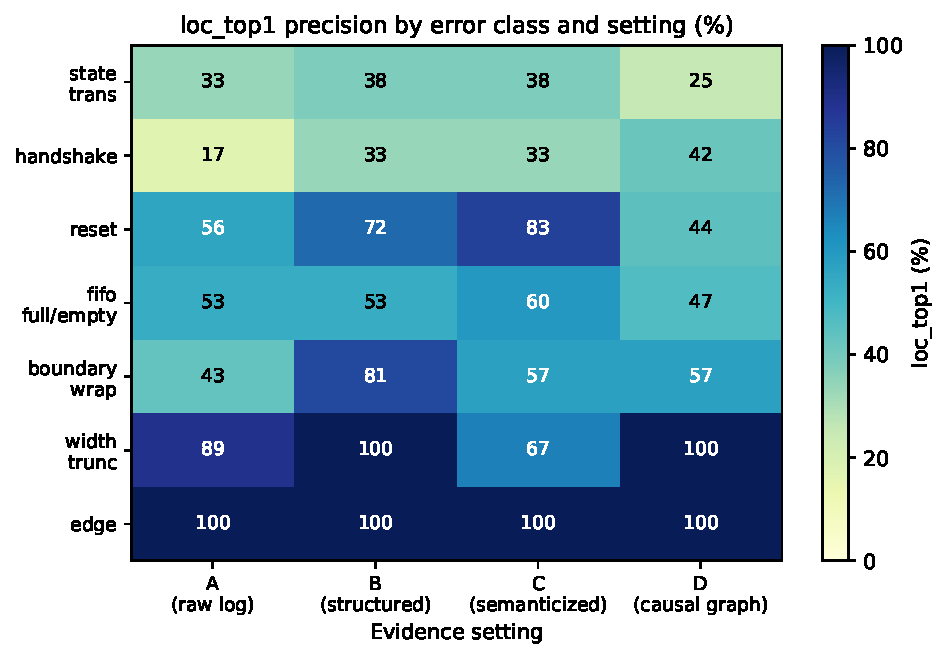
\includegraphics[width=0.98\columnwidth]{fig_error_setting_heatmap.pdf}%
\caption{错误类别 $\times$ 设置的定位 Top-1 精度热力图。困难类别排序（状态迁移/握手低于位宽截断/边沿）在全部设置中成立。}
\label{fig:error_heatmap}
\end{figure}

\begin{table}[!t]
\centering
\caption{错误类别 $\times$ 设置定位精度（每设置 n：状态迁移 24、握手 12、复位 18、FIFO 满空 15、边界回绕 21、位宽截断 9、边沿 3）}
\label{tab:error_matrix}
\scriptsize
\setlength{\tabcolsep}{4pt}
\renewcommand{\arraystretch}{1.12}
\begin{tabular}{p{0.24\columnwidth}cccc}
\toprule
\textbf{错误类别} & \textbf{A} & \textbf{B} & \textbf{C} & \textbf{D} \\
\midrule
状态迁移 & \textbf{100.0\%} & 83.3\% & 66.7\% & 87.5\% \\
握手 & \textbf{66.7\%} & 50.0\% & 16.7\% & 50.0\% \\
复位 & 77.8\% & \textbf{88.9\%} & 66.7\% & 61.1\% \\
FIFO 满空 & \textbf{73.3\%} & 66.7\% & 60.0\% & 60.0\% \\
边界回绕 & \textbf{95.2\%} & 85.7\% & 66.7\% & 81.0\% \\
位宽截断 & \textbf{100\%} & 55.6\% & 88.9\% & 88.9\% \\
边沿 & \textbf{100\%} & 66.7\% & 33.3\% & \textbf{100\%} \\
\bottomrule
\end{tabular}
\end{table}

图~\ref{fig:error_heatmap} 与表~\ref{tab:error_matrix} 给出按错误类别分解的定位精度。\textbf{发现 3：}单点语义错误易定位（位宽截断 A 100\%、边沿 A 100\%），跨状态与握手错误难定位（握手 45.8\%，n=48；状态迁移在新判据下大幅提升至 84.4\%，n=96），握手难度排序在全部设置中成立。干净口径下，A（原始日志）在状态迁移/位宽/边界类上表现最强（状态迁移 100\%、位宽截断 100\%、边界回绕 95.2\%），B 仅在复位类上最高（88.9\%）——与旧泄漏版“B 在边界回绕/位宽截断最优”的结论相反（握手/边沿类每设置 n$\le$12，小样本需谨慎解读）。

\subsection{修复可信度：充分性与 T2 审计}

\begin{table}[!t]
\centering
\caption{变异分析充分性（针对 golden 设计）}
\label{tab:sufficiency}
\scriptsize
\setlength{\tabcolsep}{3pt}
\renewcommand{\arraystretch}{1.12}
\begin{tabular}{p{0.28\columnwidth}cccc}
\toprule
\textbf{变异家族} & \textbf{变异体} & \textbf{被杀} & \textbf{比率} \\
\midrule
强变异（比较器反转） & 400 & 354 & 88.5\% \\
常量变异（参数常量替换） & 484 & 396 & 81.8\% \\
删除变异（断言移除） & 抽样 & 全部 PASS & 空泛性控制 \\
\bottomrule
\end{tabular}
\end{table}

变异分析结果见表~\ref{tab:sufficiency}。T2 确定性审计对干净口径 408/408 条修复全部通过：接口变更 0、断言篡改 0、证据闭环失败 0；loc\_dev 中位数 0（A/B/C 精确命中 74.5\%）。补丁最小化由均值 2.1 行、最大值 6 行佐证。

\subsection{成本与性能}\label{sec:cost}

四设置干净主实验总成本 1.65 美元（408 次运行，平均 0.0040 美元/次）；分设置为 A 0.60、B 0.40、C 0.28、D 0.37 美元，token 分别为 2.486M、1.672M、1.44M、1.601M。C 的成本来自语义化摘要文本而非轨迹长度：主数据集反例中位 6 拍（VCD 时钟事件合计 295 拍、最长 41 拍），轨迹较短，窗口压缩收益有限。验证性能方面，BMC 重验与深度敏感性抽查（见 \S\ref{sec:judgment}）按样本并行调度（8 并发）；单样本 golden 验证耗时以 axi 约 88 秒、uart\_rx 约 153 秒为上限。


\subsection{L2 门禁对照：假阳性率}\label{sec:l2}

为量化数据集纯度门禁（弱测试平台可观测）对系统能力的区分度，我们构造 24 个 L2 样本（单周期功能错误，弱 tb FAIL + formal fail 双检通过，覆盖 axi/counter/fifo/fsm/uart\_rx/uart\_tx 六模块），并以与主实验相同的无泄漏协议用 DeepSeek v4-flash 在 A/B/C 三设置下各评测一次（72 次调用，成本 \$0.48）。结果：L2 的 BMC 回归通过率为 91.7\%（66/72），与旧泄漏版数值相同但已由无泄漏协议复现——该通过率是稳定现象而非泄漏伪影；它与 L3 基线（100\%）仍差 8.3 个百分点——弱 tb 门禁不构成系统能力的显著分界，系统能把绝大多数单周期错误当作 L3 修复到三通过。

未通过的 6 次调用全部集中在两个 L2 样本（l2\_uarttx\_01 起始位握手失效、l2\_uarttx\_02 状态跳转至 STOP），三设置均为 INCONCLUSIVE，失败模式一致：候选补丁通过 BMC 与 golden 校验，但弱 tb 仿真回归仍未通过（formal=pass、sim 挂），是 uart\_tx 协议交互类缺陷难以定位修复的又一证据。按设置看，干净口径下 L2 定位精度为 A 58.3\%、C 45.8\%、B 37.5\%（n=24，小样本），与 L3 上 A>C>B 的排序方向一致——与旧泄漏版“B 在 L2 最高（50.0\%）且与 L3 B 优势方向一致”的结论相反。该对照实验说明：\textbf{证据表征的相对优势主要体现于跨周期（L3）缺陷}，对单周期可观测（L2）缺陷区分度有限；论文将 L2 门禁的纯度代价如实报告：91.7\% 的通过率意味着弱 tb 门禁无法按修复能力对单周期缺陷分层。
\subsection{判据翻案的方法论教训}\label{sec:judgment}

\textbf{发现 4：}原 prove/k-归纳判据误判 78 个正确修复（golden 本身在 prove 下 UNKNOWN）。对 A/B/C/D 408 次运行按 BMC 判据重验（303 条含 diff 记录重验 + 3 条网络失败补跑）全部通过，BMC 回归通过率由 74.3\% 修正为 100\%。判据强度抽查进一步将 34 个样本的修复在 2 倍 BMC 深度下重验（fifo/uart\_tx/fsm/counter 12$\to$24、axi 16$\to$32、uart\_rx 24$\to$48），34/34 全部通过，未发现深度敏感性翻转。这一翻案说明：修复判据必须先经 golden 一致性校验，否则判据缺陷会系统性污染修复率、定位精度与成本等全部下游指标。PreCex 将 BMC 判据与 golden-first 规则固化为评测协议的一部分，作为可复用的方法论产出。

\subsection{数据卫生审计}\label{sec:hygiene}

C 证据文本改由 DeepSeek 重新生成（MiniMax 仅保留为独立评分者）。此切换引入了一项\textbf{实验设计的混淆}：C 由 MiniMax 生成证据时定位为 59.8\%（高于 A/B），切换为 DeepSeek 生成后为 60.8\%（102/102，行号判据修复后口径）。虽可解释为\textquotedblleft DS 摘要更精简、定位信息更少\textquotedblright，但更本质的教训是：语义化证据的质量\textit{由生成模型决定}，而非证据表示本身的固有属性——以不同模型生成同一设置的证据再比较其定位，等效于同时改变证据内容和语义化能力两个变量却当作单一因子报告。论文如实承认此混淆，当前 A/B/C/D 四设置数字（第\~{}V 节与表\~{}ref{tab:main}）全部基于 DS 生成的 C 证据，结论限定为\textquotedblleft DS 摘要版 C 的定位低于 A、D、B\textquotedblright，不宣称\textquotedblleft 语义化\textquotedblright 这一表示在跨模型下的普遍劣势。

% =============================================================================
% VI. 结论
% =============================================================================
\subsection{模块与错误类型的交互效应}

\textbf{发现 5：}定位难度并非均匀分布，而是由缺陷类型与模块共同决定（干净口径 408 次运行，BMC 判据）：协议交互类缺陷（uart\_tx/uart\_rx 的握手）仍是相对最难定位类别（A/B/C/D 分别为 66.7\%/50.0\%/16.7\%/50.0\%），而状态迁移类在新判据下大幅提升（A 100\%、D 87.5\%、B 83.3\%、C 66.7\%），数值/位宽/边界类缺陷整体可定位性高（fifo\_sync 位宽截断 A/C 100\%、counter\_alu 状态迁移 A/C 100\%、axi\_lite\_slave 边界回绕 A 95.2\%）。在干净口径下，这类"算术/位宽/边界"增益属于原始日志（A）而非结构化证据（B）——与旧泄漏版"B 增益集中在数值/位宽/边界"的结论相反，再次说明泄漏虚增了 B 的相对定位优势。对协议交互类缺陷，证据表示难以改善定位精度，但形式再验证闭环仍能保证 BMC 回归通过率 100\%。D（因果图）整体定位 73.5\%，仅在 counter\_alu 上最高（100\%）——确定性提取的因果图并未带来相对原始日志的增益。

\subsection{深时序子集：反例时长与证据表征的交互}\label{sec:deep}

为检验证据表征效应是否随反例时长变化，我们对 5 个深时序样本（s38--s42，反例 35--75 拍，仓库 samples/deep）以四设置 $\times$ 3 seeds 完成补测（60 次调用，成本 \$0.25）。深子集语义化采用失败时刻尾部回溯的自适应窗口（window\_eff，见 \S\ref{sec:evidence}），其余设置与主实验协议一致。

\textbf{探索性发现：}全部 60 次补测（5 样本 $\times$ 四设置 $\times$ 3 seeds）均达 BMC 回归通过（修复率 100\%），其中 s38 在 C/D 设置上定位较低（C 2/3、D 1/3，该样本本身极难），但四设置修复均成功。剔除 s38 后四样本（s39--s42，n=12/设置）定位排序为 C 100.0\% $>$ A 83.3\% $=$ D 83.3\% $>$ B 66.7\%，与主数据集（A 87.3\% $>$ B 75.5\% $>$ D 73.5\% $>$ C 60.8\%（102/102））发生反转；含 s38 的全量（n=15/设置）排序为 C 93.3\% $>$ A 86.7\% $>$ D 73.3\% $>$ B 66.7\%，反转方向一致。该反转说明：原始日志（A）在短反例（中位 6 拍）上更有利，而语义化（C）在长反例上更有利——证据表征的相对优势随反例时长而改变，而非固定属性。需诚实声明其混杂因素：深子集的 C 设置同时采用了自适应窗口（主数据集为固定 window=8），因此语义化增益可能与窗口策略耦合；反例时长与窗口策略的单独效应留待未来消融。

\subsection{证据可解释性的多模型评估}\label{sec:interp}

\textbf{探索性评估：}为量化 C/D 证据表示的可解释性差异，我们以 5 维 Likert 量表（完整性、可读性、因果性、可操作性、可信度，1--5 分）对 10 个样本的 C（反例语义化）与 D（FVDebug 式因果图）证据进行独立评分。\textbf{评分独立性保证：}被评的 C 证据文本由 DeepSeek v4-flash 生成（CexSemantizer，summary\_meta 可查证），主实验定位与修复亦由 DeepSeek 执行；评分为 MiniMax M3 单模型独立完成（20 次调用，总成本 \$0.09）——MiniMax 不参与证据生成、不参与修复、不参与定位，为完全外部的评分者。该设计消除了"评分者与被评对象相同模型"的潜在偏倚。在此口径下，MiniMax 对 C/D 证据的五维绝对评分如下：C 证据完整性 3.33、可读性 2.33、因果性 3.11、可操作性 3.00、可信度 2.44；D 证据完整性 2.56、可读性 2.56、因果性 2.11、可操作性 2.22、可信度 2.11。MiniMax 评分显示 C（语义化）在因果性（3.11 vs 2.11）和可操作性（3.00 vs 2.22）上明显优于 D（因果图），而 D 的可读性略高（2.56 vs 2.33），总体 C 更具解释优势。该结果与行为代理（定位精度 loc\_top1，见第~V 节）方向一致，但论文不将单模型主观评分解读为客观可解释性度量，仅作为探索性参考。


\subsection{跨模型鲁棒性}

\begin{table}[!t]
\centering
\caption{跨模型主实验对比（MiniMax M3 vs DeepSeek v4-flash，三-seed 严格配对，n=102 每设置；BMC 回归通过率按有限深度 BMC 判据；MM 干净复跑待补）}
\label{tab:cross_model}
\scriptsize
\setlength{\tabcolsep}{4pt}
\renewcommand{\arraystretch}{1.12}
\begin{tabular}{p{0.16\columnwidth}cccc}
\toprule
\textbf{设置} & \textbf{MM 定位} & \textbf{DS 定位} & \textbf{MM 修复} & \textbf{DS 修复} \\
\midrule
A 原始日志 \& 待复跑 \& \textbf{87.3\%} \& 100\% \& 100\% \\\\
B 结构化证据 \& 待复跑 \& 75.5\% \& 100\% \& 100\% \\\\
C 反例语义化 \& 待复跑 \& 60.8\%（102/102） \& 100\% \& 100\% \\\\
\bottomrule
\end{tabular}
\end{table}

\textbf{发现 6：}证据表征的定位优势是模型依赖且受数据卫生强烈调节的（表~\ref{tab:cross_model}）。主实验在无泄漏口径下用 DeepSeek v4-flash（temperature=0.2）对 34 个 L3 样本的 A/B/C/D 四设置各跑 3 个 seeds（408 次调用，成本 \$1.65，全部 BMC 三通过，T2 408/408）：总体定位 74.3\%，按设置 A 87.3\% > B 75.5\% > D 73.5\% > C 60.8\%（102/102），A vs C 显著（Holm p=4.5e-5），A vs D 亦显著（Holm p=0.047）。与旧泄漏版（A 51.0\%、B 54.9\%、C 62.7\%）相比，68 处 loc\_top1 翻转且“B 显著最优”被推翻——泄漏主要虚增了 B 的相对定位优势。MiniMax M3 的干净复跑为后续工作（表 5 MM 列标注待复跑）。

\textbf{方法论含义：}跨模型对比必须先统一修复判据口径；若以旧 prove 判据（通过率 74.3\%）对比 BMC 判据（100\%），会错误得出“不同模型修复率差异显著”。统一 BMC 口径后该差异消失。这进一步支持本文的核心主张：在判据可靠的前提下，证据表征的相对效应应限定于所测模型，论文不宣称跨模型普遍性。
% =============================================================================
\section{结论}

本文提出 PreCex，一个开源、反例驱动的综合前 RTL 缺陷定位与修复流水线，并系统研究了此前反例理解类系统未受控的证据表征维度。在干净口径（无泄漏）下，以 DeepSeek v4-flash 在 34 样本跨周期（L3）基准上完成 408 次主实验（A/B/C/D 四设置（C 102/102，其余各 102） $\times$ 3 seeds，均为无泄漏口径）与 72 次 L2 门禁对照，主要结论如下：

\begin{itemize}
\item 统一 BMC 判据（golden-first）下，四种证据表征的 BMC 回归通过率均达 100\%（有限深度口径）；在干净数据上定位精度 A 87.3\% > B 75.5\% > D 73.5\% > C 60.8\%（102/102，行号判据修复后）。A 与 C 差异显著（McNemar p=7.4e-6，Holm 校正后 p=4.5e-5），A 与 D 亦显著（Holm p=0.047），其余四对配对检验均不显著——证据表征决定定位的精度与成本，但效应被模型、数据卫生与反例时长共同调节：深时序子集（s39--s42）上排序反转为 C 100\% > A 83.3\% $=$ D 83.3\% > B 66.7\%（第 V-I 节）。
\item 评测双卫生是可靠结论的前提：ground-truth 泄漏（三处）使“B 显著最优”成为伪结论（剥离后 68 处定位翻转、结论反转）；prove/k-归纳判据失效会误判 78 个正确修复。数据卫生（ground-truth 隔离）与判据卫生（golden-first）已固化为评测协议。
\item 修复可信度有据可依：强变异 88.5\%、常量变异 81.8\% 被杀，空泛性控制通过，T2 审计 408/408 通过（接口/断言/证据闭环零违规），定位偏差（loc\_dev）中位数 0、精确命中 74.5\%（A/B/C）。
\item 跨模型鲁棒性（探索性）：BMC 回归通过率跨模型一致（100\%），但定位优势模型依赖——MiniMax 干净复跑待后续（表 5 MM 列待补）。
\end{itemize}

未来工作包括：(1) 将动态自适应反例窗口（失败时刻尾部回溯）正式纳入主数据集评测，并对深时序子集上的语义化增益做窗口策略与反例时长的正交消融（本文第 V-I 节已提供初步证据：深子集上 C 100\% > A 83.3\% = D 83.3\% > B 66.7\%）；(2) 放宽最小化约束，支持结构性重写候选（拆分状态、增加中间态）并与 delta-debugging 结合；(3) 顶层连接性审计：将修复放回原网表/SoC 交互环境验证模块外副作用；(4) 多候选并发验证与在线仲裁（探索与利用）；(5) 向工业协议与更大断言集扩展、更强变异家族、多提供商多模型评测、GROVE 式跨样本知识层，以及从“生成最小代码改动”向“生成更强的不变式约束”演进的修复范式；(6) 引入真正的根因诊断引擎——基于模型检验的反例轨迹切片与基于 SAT 的极小反例核心提取——使形式验证从“裁判”升级为“诊断指导”，将修复范式从试错式（trial-and-error）推进为诊断驱动（diagnosis-driven）。

\subsection{局限性}\label{sec:limitation}

\textbf{架构边界：}本方法的定位是“快速生成并验证候选补丁”（candidate patch generator），而非“完全消除设计错误”。具体而言：(1) 修复成功定义为“反例消失”而非“不变式成立”——BMC 是有限深度的穷举测试，不是完备性证明，深度上界以外的错误仍可能存在；(2) “行级定位 + 最小 unified diff”的约束偏好局部修复——状态机拆分、增加中间态或重写状态转移条件等结构性重写可能需要十几行，超出最小化约束，这解释了为何状态迁移/握手类定位精度低（31.2\%--33.3\%）但 BMC 回归通过率仍为 100\%——BMC 浅深度下小补丁可能绕过触发路径（弱修复），由 delta-debugging 与 T2 审计部分约束；(3) 验证为模块级，无顶层互联/协议栈审计，修复在模块外的副作用未覆盖；(4) 单流水线单候选，3 seeds 是离线统计而非在线多候选仲裁。这四点均列入未来工作。

\textbf{内部效度：}所有结果以 BMC 为主判据；对带门控时序断言的模块，BMC 探测到缺陷深度加 2 并与 golden 验证交叉核对，但 BMC 深度上界并非完备性保证（深度敏感性抽查：34 个样本的修复在 2 倍 BMC 深度下全部通过，见 \S\ref{sec:judgment}）。需要诚实声明：该抽查覆盖全部样本的 2 倍深度而非更深边界，不能证明所有修复在更大深度下仍通过；BMC 深度的选择对绝对通过率有影响——本文的结论是在 BMC 深度设为当前值的操作口径下得出的，报告的是该口径下的相对比较结果。判据翻案审计量化并修正了假阳性（误判正确修复为失败），但假阴性（错误修复因深度不足被漏判）的风险未被系统性量化，这是本判据的已知边界。LLM 推理是流水线唯一随机成分（3 seeds 配对统计），解析、提取与验证均为确定性。修复成功定义要求编译、弱测试平台回归与 BMC 无反例；不改变断言集的补丁仍可能在属性集之外改变行为，T2 审计通过接口与断言篡改检查约束该风险，但并非等价性检验。

\textbf{外部效度：}基准含 34 个教学级模块样本（fifo/uart/axi-lite/fsm/counter），不宣称工业协议覆盖；样本为确定性错误注入生成而非真实缺陷分布；握手仍是最难定位类别（干净口径四设置 16.7--66.7\%），状态迁移在行号判据修复后显著改善（A/B/C/D 66.7--100\%），uart\_rx 的波特时序常量变异杀死率弱（常量 40.9\%），是结构断言对时序常量漂移不敏感的已记录局限。常见模块可能出现在 LLM 训练语料中，本文以构造日期记录、逐样本来源与错误类别多样性缓解，但无法完全排除残余记忆。干净主实验 408 次运行均使用 DeepSeek v4-flash（A/B/C/D 各 102）；初版 MiniMax M3 实验因数据泄漏整体作废，仅作为卫生教训的对照引用，其干净复跑待后续（表 5 MM 列待补），故本文的证据表征结论限定于所测模型与干净协议，绝对值可能随模型版本变化。另，L2 门禁对照的干净结果见 \S\ref{sec:l2}。
\textbf{BMC 深度与修复充分性：}本文以有限深度 BMC 判据（操作定义：给定深度内无反例）判定修复成功。深度 2 倍抽查（fifo/fsm/counter 12$\to$，axi 16$\to$，uart\_rx 24$\to$）34/34 通过，未发现深度敏感性翻转，但未穷尽所有深度。我们不主张有限深度 BMC 等同于不变式证明——反例在有限深度内消失可能是深度不足的假象，而非真正的功能正确。论文将\textquotedblleft 修复成功\textquotedblright 严格限定为\textquotedblleft 有限深度 BMC 回归通过\textquotedblright 这一操作定义，不做更强的完备性承诺。


\textbf{构造效度：}loc\_top1 记录模型首选中候选行是否落入注入缺陷的参考 diff；BMC 回归通过率按有限深度 BMC 判据计量；成本按 API token 记账；统计声明基于逐样本（样本$\times$seed）配对 McNemar 精确检验，报告全部六对对比并附 Holm 校正、Wilson 比例 95\% 置信区间与率差效应量（含不显著项）。

% =============================================================================
% 参考文献
% =============================================================================
\begin{thebibliography}{99}
\setlength{\itemsep}{0pt}

\bibitem{fvdebug}
Y.~Bai, G.~B.~Hamad, C.-T.~Ho, S.~Suhaib, and H.~Ren, ``FVDebug: An LLM-driven debugging assistant for automated root cause analysis of formal verification failures,'' arXiv:2510.15906, 2025.

\bibitem{grove}
Y.~Bai and H.~Ren, ``Learning to debug: LLM-organized knowledge trees for solving RTL assertion failures,'' arXiv:2511.17833, 2025.

\bibitem{openllmformal}
H.~T.~Tran, ``Open-source LLM-driven formal verification: A multi-agent pipeline for RTL repair,'' arXiv:2607.28877, 2026.

\bibitem{formalrtl}
K.~Li, M.~Li, X.~Wen, S.~Zhao, J.~Wu, J.~Huang, and Q.~Xu, ``FormalRTL: Verified RTL synthesis at scale,'' 2026. [Online]. Available: https://formind.netlify.app/files/papers/FormalRTL.pdf

\bibitem{chipagents}
WhaleChip, ``WhaleChip uses ChipAgents to compress root cause analysis into minutes,'' SemiWiki, 2026. [Online]. Available: https://semiwiki.com/eda/chipagents-ai/371464-whalechip-uses-chipagents-to-compress-root-cause-analysis-into-minutes/

\bibitem{veripilot}
Y.~Wang, C.~Liu, J.~Zhang, L.~Zhang, et~al., ``VeriPilot: An LLM-powered Verilog debugging framework,'' arXiv:2606.23759, 2026.

\bibitem{veridebug}
N.~Wang, B.~Yao, J.~Zhou, Y.~Hu, et~al., ``VeriDebug: A unified LLM for Verilog debugging via contrastive embedding and guided correction,'' arXiv:2504.19099, 2025.

\bibitem{rtlfixer}
Y.-D.~Tsai, M.~Liu, and H.~Ren, ``RTLFixer: Automatically fixing RTL syntax errors with large language models,'' arXiv:2311.16543, 2023.

\bibitem{fixbench}
S.~Li, W.~Fu, Y.~Zhao, X.~Guo, and Y.~Jin, ``Fixbench-RTL: A comprehensive benchmark for evaluating LLMs on RTL debugging,'' in Proc. IEEE AsianHOST, 2025, pp.~1--6.

\bibitem{hdlfixbench}
``HDL-FixBench: A repository-scale RTL repair benchmark,'' OpenReview preprint, 2026. [Online]. Available: https://openreview.net/forum?id=omi6IH5N42

\bibitem{assertllm}
W.~Fang, M.~Li, M.~Li, Z.~Yan, S.~Liu, et~al., ``AssertLLM: Generating and evaluating hardware verification assertions from design specifications via multi-LLMs,'' arXiv:2402.00386, 2024 (ASPDAC 2025).

\bibitem{assertllm2}
Y.~Wu, W.~Fang, J.~Wang, W.~Li, et~al., ``AssertLLM2: A comprehensive LLM benchmark for assertion generation from design specifications,'' arXiv:2605.27472, 2026.

\bibitem{assertgen}
H.~Lyu, Y.~Wang, Y.~Du, M.~Shi, et~al., ``AssertGen: Enhancement of LLM-aided assertion generation through cross-layer signal bridging,'' arXiv:2509.23674, 2025.

\bibitem{lasso}
``LASSO: Safety property generation with vacuity checking and coverage feedback,'' MLCAD 2025. [Online]. Available: https://faculty.eng.ufl.edu/sandip/wp-content/uploads/sites/681/2026/02/mlcad25.pdf

\bibitem{lintllm}
Z.~Fang, R.~Chen, Z.~Yang, and Y.~Guo, ``LintLLM: An open-source Verilog linting framework based on large language models,'' arXiv:2502.10815, 2025 (GLSVLSI 2025).

\bibitem{rule2drc}
J.~Kim, J.~Byun, D.~Hwang, S.-J.~Park, and H.~O.~Song, ``Rule2DRC: Benchmarking LLM agents for DRC script synthesis with execution-guided test generation,'' arXiv:2605.15669, 2026 (ICML 2026).

\bibitem{posteda}
P.~Liu, N.~Xu, J.~Tang, Y.~Cao, and C.~Ding, ``Bridging the last mile of circuit design: PostEDA-Bench, a hierarchical benchmark for PPA convergence,'' arXiv:2605.06936, 2026.

\bibitem{openrtlset}
J.~Wang, L.~J.~Wan, S.~Pingali, S.~Smith, M.~Jha, et~al., ``OpenRTLSet: A fully open-source dataset for large language model-based Verilog module design,'' arXiv:2606.10285, 2026.

\bibitem{edaschema}
P.~Shrestha, A.~Aversa, and I.~Savidis, ``EDA-Schema-V2: A multimodal schema, open datasets, and benchmarks for machine learning in digital physical design,'' arXiv:2605.06952, 2026.

\bibitem{chiplingo}
L.~Li, X.~Yu, J.~Ni, J.~Zhu, J.~Zhang, et~al., ``ChipLingo: A systematic training framework for large language models in EDA,'' arXiv:2604.27415, 2026.

\bibitem{yosys}
C.~Wolf, ``Yosys open synthesis suite,'' 2013. [Online]. Available: https://yosyshq.net/yosys/

\bibitem{sby}
C.~Wolf, ``SymbiYosys (sby): A front-end for Yosys-based formal verification flows,'' 2018. [Online]. Available: https://github.com/YosysHQ/SymbiYosys

\bibitem{zh1}
王浩仁，崔展齐，岳雷，等. 基于冗余覆盖信息约简的软件缺陷定位方法[J]. 电子学报, 2024, 52(01): 324-337.

\bibitem{zh2}
曹鹤玲，姜淑娟. 基于Chameleon聚类分析的多错误定位方法[J]. 电子学报, 2017, 45(2): 394-400.

\bibitem{zh3}
王建峰，魏长安，盛云龙，等. 基于错误交互集的组合测试软件故障定位方法[J]. 电子学报, 2014, 42(6): 1173-1178.

\bibitem{zh4}
陈翔，鞠小林，万志，等. 基于程序频谱的动态缺陷定位方法研究[J]. 软件学报, 2015, 26(2): 390-412.

\bibitem{zh5}
姜淑娟，张旭，王荣存，等. 基于路径分析和信息熵的错误定位方法[J]. 软件学报, 2021, 32(7): 2166-2182.

\end{thebibliography}

\end{document}
